\section{Looking at the big picture}
\label{sec:ch2:bigpicture}


Welcome to the Neurobiology Institute! A colleague has come to you with an interesting problem. Brains consist of neurons. Different patterns in which these neurons connect produce the unique functions your brain is able to do: it is able to manage functions like breathing, as well as more active functions like moving, hearing, seeing, and higher level thought.

When they are electrically stimulated, neurons transmit that electrical signal to other neurons. This process consumes a lot of energy for your body; while the brain is only about 2\% of your weight, it consumes about 20\% of the energy your body uses per day. To keep the neurons replenished with energy (and to remove waste that the cells produce when they work), the brain has a complicated network of blood vessels. When a brain area is in use, the body dedicates blood supply to the area that will need it most.

Neurobiologists came up with a rather clever way to decipher brain activity in humans by looking at this blood flow. Using MRI, they can trace the particular areas that the blood was flowing towards. Scientists were able to demonstrate that this signal really did tend to correlate with brain activity. 

\begin{figure}[h]
    \centering
    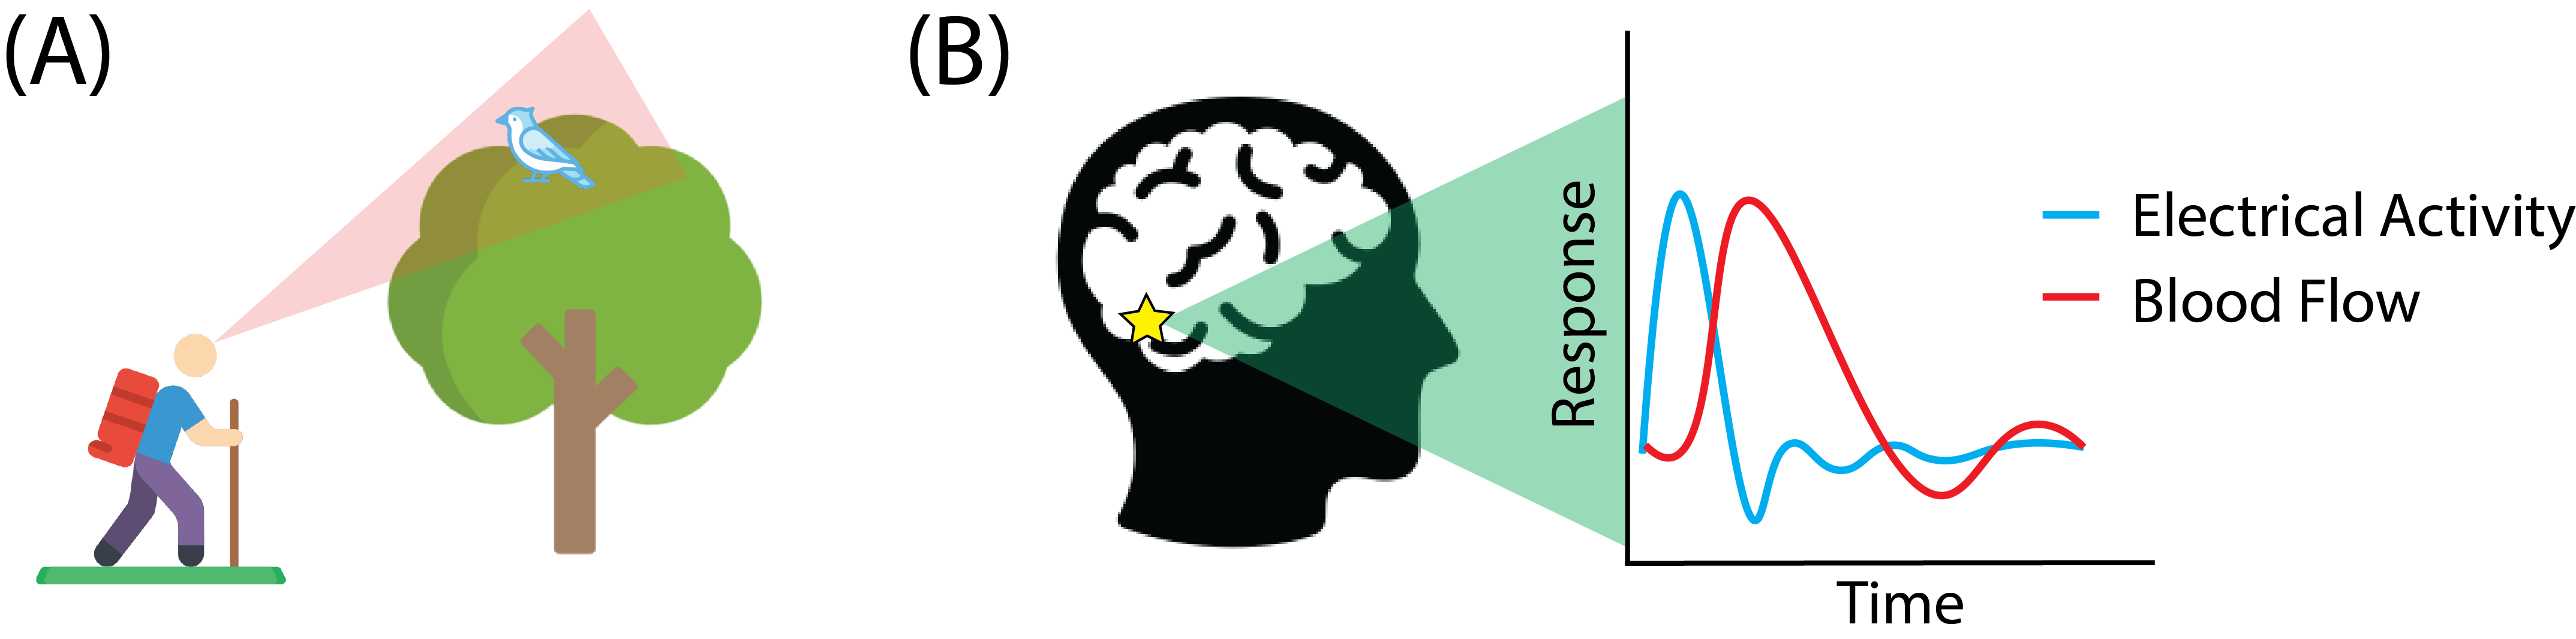
\includegraphics[width=\linewidth]{foundations/ch2/Images/fmri_bold.png}
    \caption[BOLD f-MRI]{(A) A hiker out on the trails sees a bird pirched in a tree in his field of view (faint red triangle). (B) The occipital lobe, which is responsible for sight, sits in the back of the brain (star). The presence of the bird in the field of view causes neurons to be electrically stimulated (blue line). The activity of the neurons causes the brain to send blood to the area as the neurons are stimulated (red line). While individual neurons are too small to see, the blood flow of many neurons in the brain can be picked up by the fMRI scanner.}
    \label{fig:fmri-bold}
\end{figure}

This imaging technology, known as functional MRI, has proven to be interesting to neuroscientists \cite{Poldrack2011Aug}. By measuring pairs of brain areas, researchers can see whether the two areas tend to be active together. The idea is that, perhaps, different combinations of brain areas tend to work together as a unit, allowing the complicated thought patterns that humans are capable of. By viewing the different areas of the brain as nodes of a network, and the correlations as the edges, scientists have constructed networks from this line of thinking. This area of study, called connectomics, presents an extremely network-centric area of research \cite{Munsell2018Sep}.

Your colleague has come to you with a bunch of networks from fMRI sessions, and wants to know whether there are any higher level groups of brain areas that tend to have similar activity. Can you, as a network scientist, take this network of nodes and edges, and figure out a way to break the nodes into groups of nodes which are functionally similar?

\subsection{Framing the problem}

The first question to ask your colleague is; what exactly is the objective here? In network machine learning, the choice of the model used is \emph{everything}. The model determines what sorts of questions we are capable of asking, and what sorts of \emph{answers} we are capable of learning. Asking about the objectives will directly shape which models and approaches you use.

Your colleague wants to know whether there are any sub-groups of areas that tend to behave similarly. By ``behave similarly'', what your colleague means is, are there sub-groups of brain areas that tend to work together in conjunction with other sub-groups of brain areas?

The next question is what we've tried so far. This will prevent you from repeating work, help you understand where to start approaching the problem, and give you a reference for the performance of your techniques. 

Next, you need to determine what type of network machine learning problem you have. What type of data do you have? Do you have any covariates associated with that data? What type of question do you want to answer? Do you want to test a hypothesis, or make predictions? What characteristics will your model need to reflect to be able to answer the question appropriately? Before you progress further, you should answer these questions for yourself. 

Remembering back to the types of network machine learning problems in Section \ref{sec:ch1:types}, you conclude that this is a multiple network learning problem. Your networks are non-attributed, since you only know the nodes and edges of the network. The question asks about groups of nodes and edges, and you hope to use network modelling approaches to study your problem. You are going to need to come up with a definition of what it means for pairs of areas to be similar, and you are going to want to be able to group areas in a way that is meaningful for your colleague.

\subsection{Check the assumptions}

Throughout the course of this book, we will try to keep in direct focus the assumptions being made by the techniques you might pick. You want to choose the simplest set of assumptions that can reasonably reflect the data. This means that you want to use the simplest statistical model that can answer the question you want to address. In this case, we don't care about individual brain area-to-brain area connections at all: we only care about how groups of brain areas behave in relation to other groups of brain areas. This means that we want to choose models which will allow us to learn about pairs of brain area groups, which is a very different problem from learning about individual brain areas themselves.

After talking over your understanding of the problem with your colleague, you are confident that he wants a way to be able to group brain areas together based on how similar they are, and you have the freedom to define that however you choose. You have the green light to begin coding!

\newpage